\pdfminorversion=7
\documentclass[14pt]{beamer}

\usepackage[utf8]{inputenc}
\usepackage[english]{babel}
\usepackage[T1]{fontenc}
\usepackage{newtxmath}
\usepackage[
bibstyle=authoryear, % alphabetical
citestyle=authoryear, % alphabetical
backend=biber,
maxnames=2,
maxbibnames=99]{biblatex}
\addbibresource{literature.bib}
\AtBeginBibliography{\tiny}
\usepackage{graphicx}
\usepackage{xcolor}
\usepackage{url}
\usepackage{pifont}
\usepackage{booktabs}
\usepackage{amsmath}
\usepackage{mathtools}
\usepackage{bbm}
\usepackage[mathcal]{euscript}
\usepackage{geometry}
\usepackage{listings}
\usepackage{cancel}
\usepackage{multimedia} % videos
\usepackage{layouts}

\beamertemplatenavigationsymbolsempty
\setbeamerfont{page number in head/foot}{size=\large}
\setbeamertemplate{footline}{%
\hfill%
\usebeamercolor[fg]{page number in head/foot}%
slide
\usebeamerfont{page number in head/foot}%
\insertframenumber%
\kern2pt\vskip1pt%
}

\definecolor{backcolor}{rgb}{0.2,0.2,0.2}
\definecolor{keycolor}{rgb}{0.8,0.471,0.196}
\definecolor{codecolor}{rgb}{0.9,0.9,0.9}
\definecolor{stringcolor}{rgb}{0.416,0.718,0.349}
\definecolor{commentcolor}{rgb}{0.5,0.5,0.5}
\lstdefinestyle{pythonstyle}{
    backgroundcolor=\color{backcolor},
    keywordstyle=\color{keycolor},
    commentstyle=\color{commentcolor},
    %numberstyle=\tiny\color{codegray},
    stringstyle=\color{stringcolor},
    basicstyle=\ttfamily\scriptsize\color{codecolor},
    breakatwhitespace=false,
    breaklines=true,
    captionpos=b,
    keepspaces=true,
    showspaces=false,
    showstringspaces=false,
    showtabs=false
}

\lstset{style=pythonstyle}

\begin{document}

\begin{frame}[plain,noframenumbering]
\begin{center}
{\usebeamercolor[fg]{title}\usebeamerfont{title}Transformations in Three Dimensions\par}
\vfill

\setbeamercolor{boxcolor}{bg=blue!5}
\begin{beamercolorbox}[sep=0.5em,center]{boxcolor}
\textbf{Alexander Fabisch}\\
DFKI GmbH, Robotics Innovation Center
\end{beamercolorbox}

\vfill
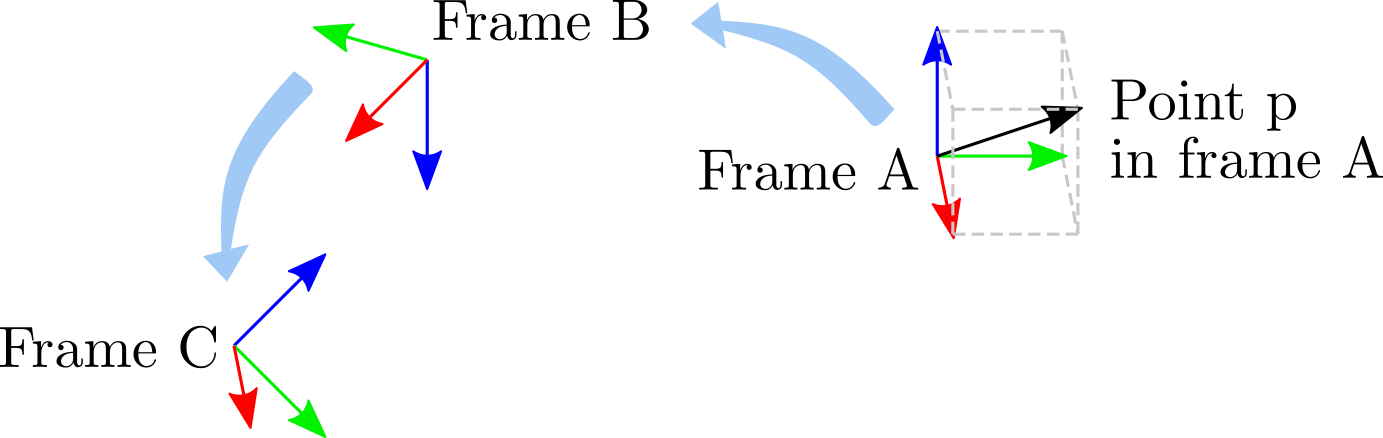
\includegraphics[width=\textwidth]{images/transformation_modeling}
\vfill
\url{https://github.com/dfki-ric/pytransform3d}
\end{center}
\end{frame}

\begin{frame}

\includegraphics[width=\textwidth]{images/logo}
\setbeamercolor{boxcolor}{bg=green!10}
\begin{beamercolorbox}[wd=\textwidth,sep=1em]{boxcolor}
\textbf{git}

{\small \url{https://github.com/dfki-ric/pytransform3d}}
\end{beamercolorbox}

\setbeamercolor{boxcolor}{bg=blue!10}
\begin{beamercolorbox}[wd=\textwidth,sep=1em]{boxcolor}
\textbf{Citation}

\textcite{Fabisch2019}. \textit{pytransform3d: 3D Transformations for Python}. Journal of Open Source Software, 4(33), 1159.
\end{beamercolorbox}
\end{frame}

\begin{frame}{Overview}
\begin{itemize}
\item Introduction to 3D Rigid Transformations
\item Applications
\begin{itemize}
\item Imitation Learning
\item Concatenation of Uncertain Transforms
\item Transfer of Motions to Robotic Hands
\item Collision Detection
\end{itemize}
\end{itemize}
\end{frame}

\begin{frame}
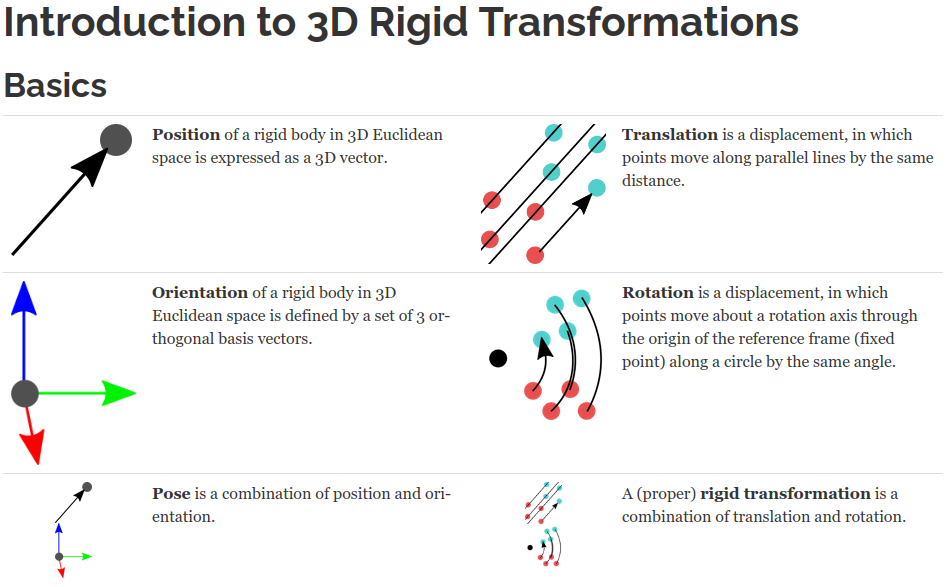
\includegraphics[width=\textwidth]{images/introduction}
\end{frame}

\begin{frame}{Frames}
A \textit{coordinate reference} \textbf{frame} in 3D Euclidean space is defined by an origin (position) and 3 orthogonal basis vectors (orientation) and it is attached to a rigid body.

\vfill

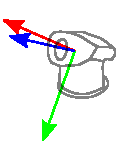
\includegraphics[height=1.9cm]{images/conventions_camera}
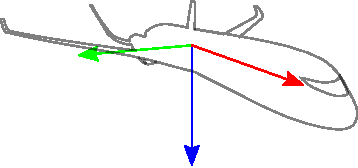
\includegraphics[height=1.9cm]{images/conventions_plane}
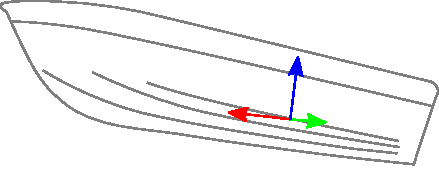
\includegraphics[height=1.9cm]{images/conventions_ship}

\vfill

\setbeamercolor{boxcolor}{bg=blue!10}
\begin{beamercolorbox}[wd=\textwidth,sep=1em]{boxcolor}
We will use RGB lines to indicate basis vectors.
\end{beamercolorbox}
\end{frame}

\begin{frame}
\begin{center}
\Large
Application: Imitation Learning
\end{center}
\end{frame}

\begin{frame}[fragile]{Imitation Learning}
\begin{columns}
\begin{column}{0.43\textwidth}
\makebox(129.5,143.75){
\movie[autostart,poster,width=129.5pt]
{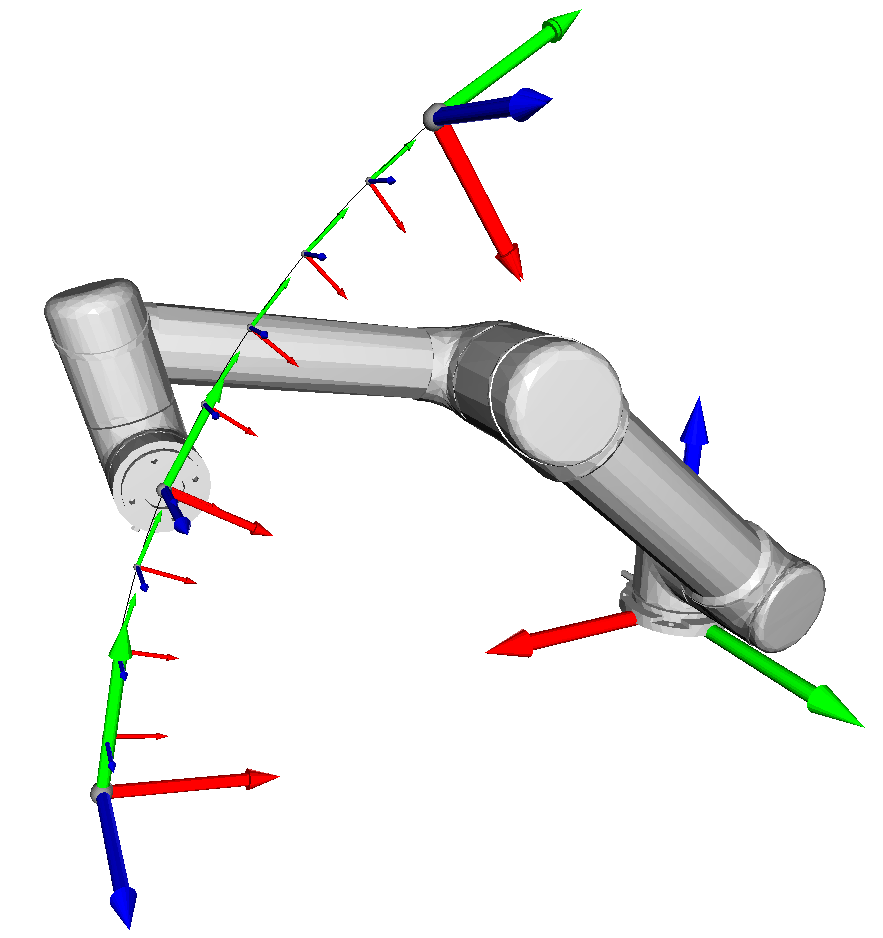
\includegraphics[width=129.5pt,height=143.75pt]{images/movement_primitives_cart_dmp_ur5}}
{videos/movement_primitive.mp4}}
\end{column}
\begin{column}{0.55\textwidth}
\textbf{Given:} one or more solutions to a problem (trajectories)\\[1em]

How can we represent orientation?
\end{column}
\end{columns}

\vfill

\setbeamercolor{boxcolor}{bg=blue!10}
\begin{beamercolorbox}[wd=\textwidth,sep=5pt]{boxcolor}
{\footnotesize Library:
\url{https://github.com/dfki-ric/movement_primitives}}
\end{beamercolorbox}
\end{frame}

\begin{frame}{SO(3) (SO: special orthogonal group)}
--- group of all rotations in 3D

--- represented by 3D rotation matrices

\vfill

\begin{center}
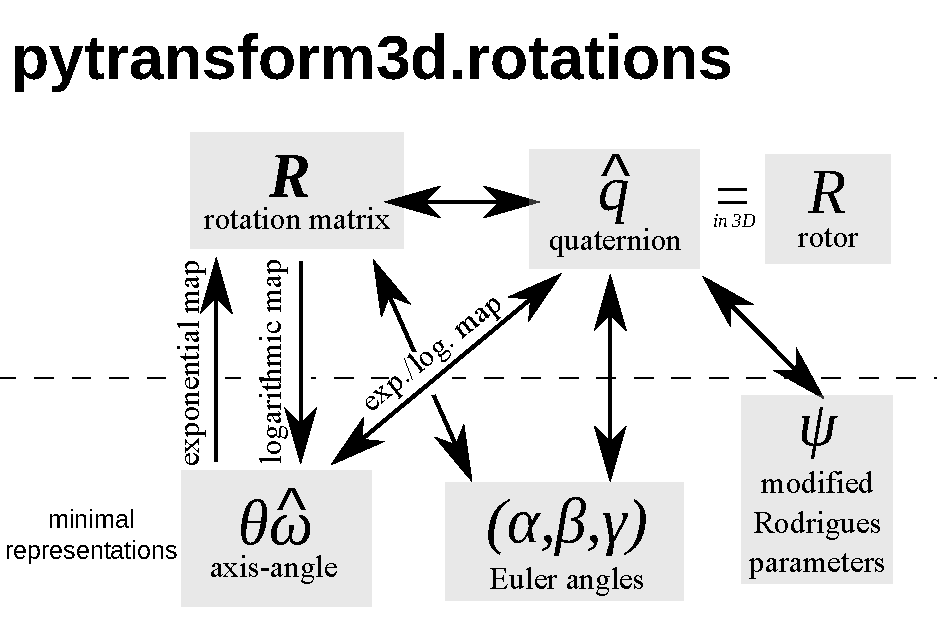
\includegraphics[width=9cm]{images/rotations}
\end{center}
\end{frame}

\begin{frame}[fragile]{Imitation Learning}
\begin{columns}
\begin{column}{0.3\textwidth}
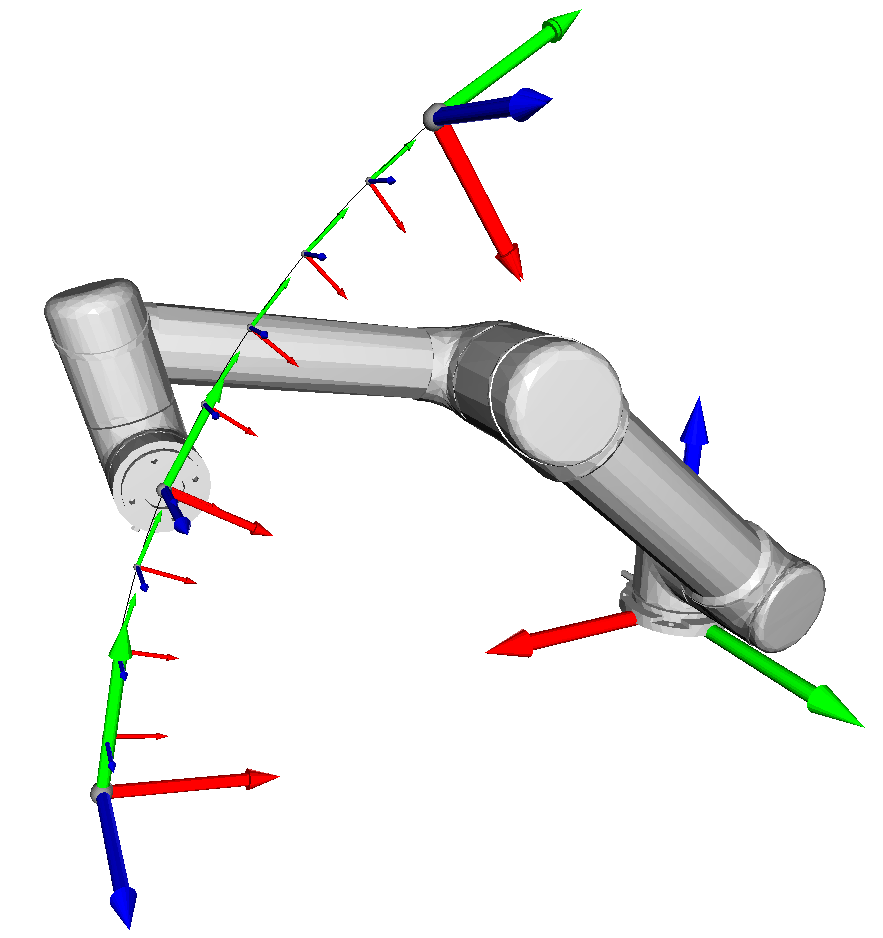
\includegraphics[width=\textwidth]{images/movement_primitives_cart_dmp_ur5}
\end{column}
\begin{column}{0.7\textwidth}
Problems
\begin{itemize}
\item Rotation matrices have 6 constraints that are not easy to enforce
\item Minimal representations $\in \mathbb{R}^3$ have singularities
\item Quaternions $q \in \mathbb{S}^3$ have an ambiguity: $q = -q$
\end{itemize}
\end{column}
\end{columns}
\end{frame}

\begin{frame}[fragile]{Quaternions - Pitfalls}
We want to use quaternions \parencite{Ude2014}

\vskip 1cm
\pause

Be careful:
\begin{itemize}
\item Quaternions $q \in \mathbb{S}^3$ have an ambiguity: $q = -q$
\begin{lstlisting}[language=Python]
from pytransform3d.rotations import pick_closest_quaternion
q1 = pick_closest_quaternion(q1, q2)
\end{lstlisting}
\item 2 conventions: \textbf{Hamilton} vs. JPL\\\parencite{Sommer2018}
\item 4 numbers, e.g., $(0, 1, 0, 0)$\\
-- \textbf{scalar first} $(\textcolor{red}{w}, x, y, z)$ or last
$(x, y, z, \textcolor{red}{w})$
\end{itemize}
\end{frame}

\begin{frame}[fragile]{Visualizer -- matplotlib-like interface}
\begin{columns}
\begin{column}{0.3\textwidth}
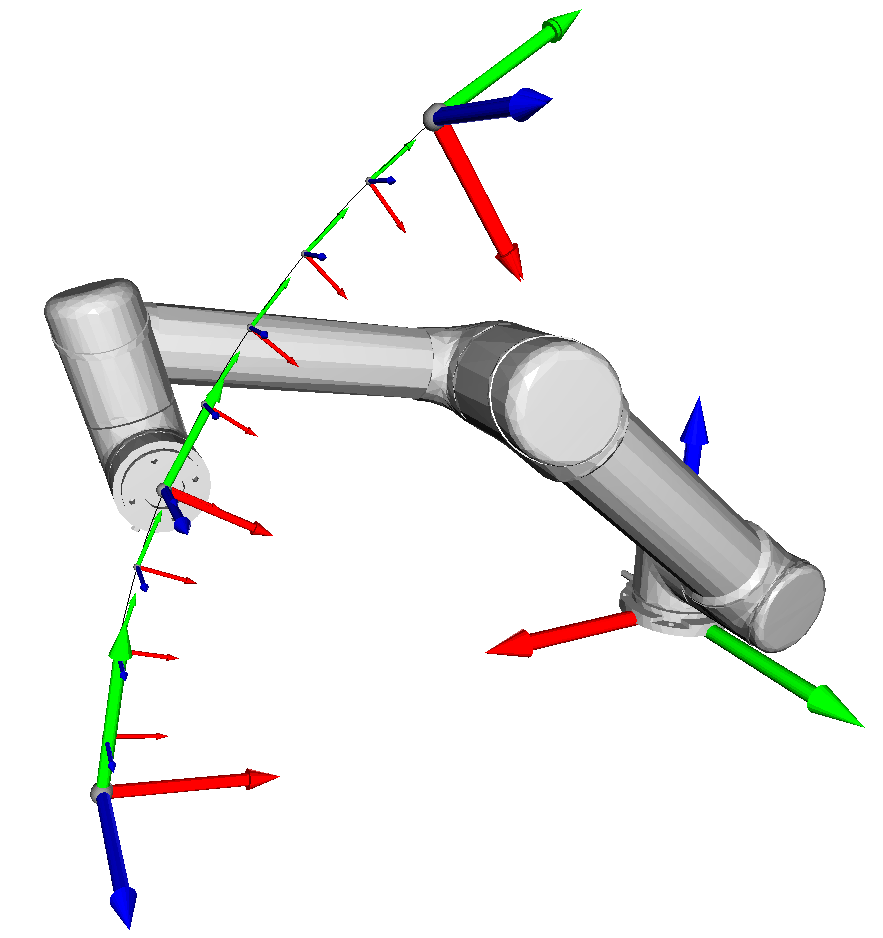
\includegraphics[width=\textwidth]{images/movement_primitives_cart_dmp_ur5}
\end{column}
\begin{column}{0.7\textwidth}
\begin{lstlisting}[language=Python]
import pytransform3d.visualizer as pv


fig = pv.figure()
fig.plot_transform(s=0.3)

fig.plot_graph(
    urdf_transform_manager,
    "ur5_base_link",
    show_collision_objects=True,
    show_frames=True)

fig.plot_transform(ee2base_start)
fig.plot_transform(ee2base_end)

pv.Trajectory(trajectory).add_artist(fig)

fig.view_init()
fig.show()
\end{lstlisting}
\end{column}
\end{columns}
\end{frame}

\begin{frame}
\begin{center}
\Large
Application: Concatenation of Uncertain Transforms
\end{center}
\end{frame}

\begin{frame}[fragile]{Probabilistic Robot Kinematics}
\makebox(224.3,167.5){
\movie[loop,autostart,poster,width=224.3pt]
{\makebox(224.3,167.5){}}
{videos/prob_robot_kin.mp4}}

\vskip 1em

\setbeamercolor{boxcolor}{bg=blue!10}
\begin{beamercolorbox}[wd=\textwidth,sep=5pt]{boxcolor}
Examples $>$ 3D Visualizations $>$ Probabilistic Product of Exponentials
\end{beamercolorbox}
\end{frame}

\begin{frame}[fragile]{Concatenation of Uncertain Transforms}
\begin{center}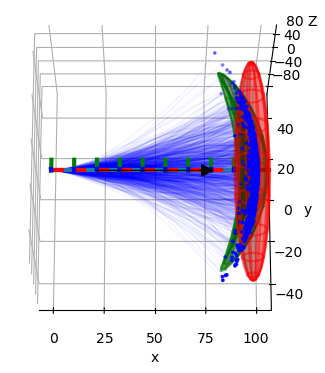
\includegraphics[width=0.4\textwidth]{images/state_estimation}\end{center}
\vskip -0.4cm
\begin{itemize}
\item Uncertainty of angular velocity about z-axis
\item \textcolor{blue}{Blue}: Monte Carlo sampling of trajectories
\item \textcolor{red}{Red}: Gaussian of MC-sampled final positions
\item \textcolor{green}{Green}: Propagated uncertainty in \textit{exponential coordinates}
(\textbf{banana distribution})
\end{itemize}
\end{frame}

\begin{frame}{SE(3) (SE: special Euclidean group)}
--- group of all proper rigid transformations in 3D

--- represented by transformation matrices

\vfill

\begin{center}
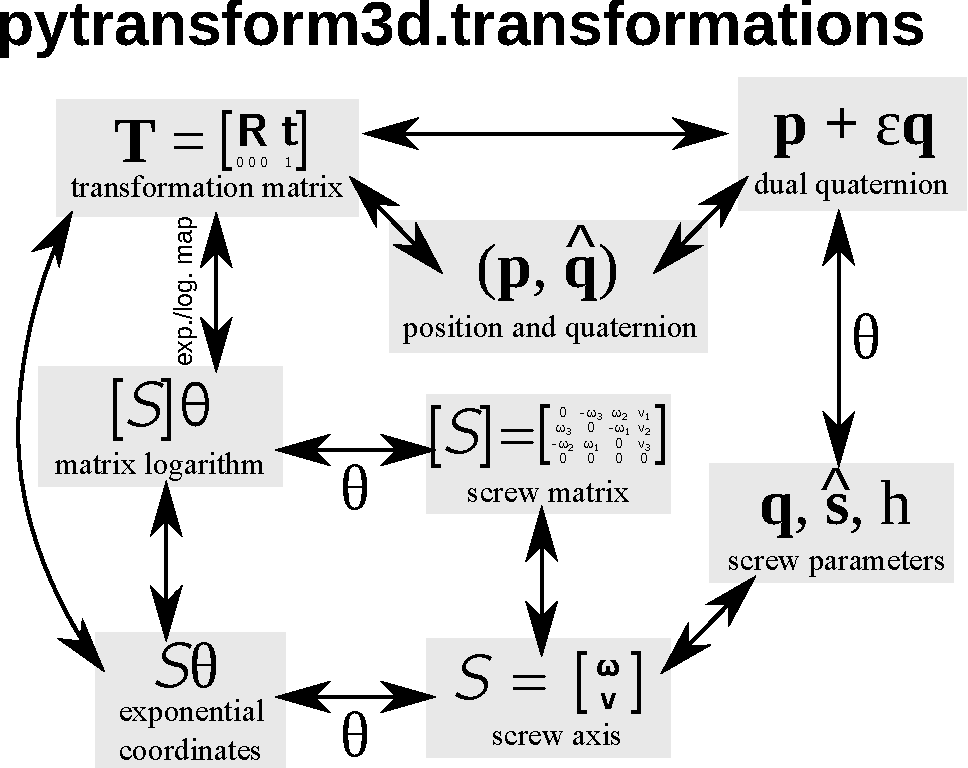
\includegraphics[width=7cm]{images/transformations}
\end{center}
\end{frame}

\begin{frame}{Transformation Matrices}
\[
SE(3) = \biggl\{ \boldsymbol{T} = \left(
\begin{array}{cc}
\boldsymbol{R} & \boldsymbol{t}\\
\boldsymbol{0} & 1
\end{array}
\right) \in \mathbb{R}^{4 \times 4}
| \boldsymbol{R} \in SO(3), \boldsymbol{t} \in \mathbb{R}^3 \biggr\}
\]

\[
\left( \begin{array}{cc}
    \boldsymbol R & \boldsymbol t\\
    \boldsymbol 0 & 1\\
\end{array} \right)
=
\left(
\begin{matrix}
r_{11} & r_{12} & r_{13} & t_1\\
r_{21} & r_{22} & r_{23} & t_2\\
r_{31} & r_{32} & r_{33} & t_3\\
0 & 0 & 0 & 1\\
\end{matrix}
\right)
\]
\end{frame}

\begin{frame}{Exponential Coordinates}
\setbeamercolor{boxcolor}{bg=blue!10}
\begin{beamercolorbox}[wd=\textwidth,sep=1em]{boxcolor}
Screw axis: $\left[ \begin{array}{c}\hat{\boldsymbol{s}} \\ \boldsymbol{q} \times \hat{\boldsymbol{s}} + h \hat{\boldsymbol{s}}\end{array} \right] = \textcolor{red}{\mathcal{S}} \in \mathbb{R}^6$
\end{beamercolorbox}

\vfill

\hfill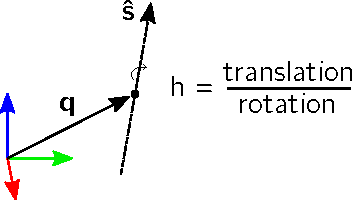
\includegraphics{images/screw_axis}

\vfill

\begin{beamercolorbox}[wd=\textwidth,sep=1em]{boxcolor}
Exponential map: $Exp(\textcolor{red}{\mathcal{S}\theta}) = \boldsymbol{T}
% =
% \left( \begin{array}{cc}
% \boldsymbol R & \boldsymbol t\\
% \boldsymbol 0 & 1\\
% \end{array} \right)
\in SO(3)$
\end{beamercolorbox}

\parencite{Lynch2017}
\end{frame}

\begin{frame}[fragile]{Concatenation of Uncertain Transforms}
\begin{center}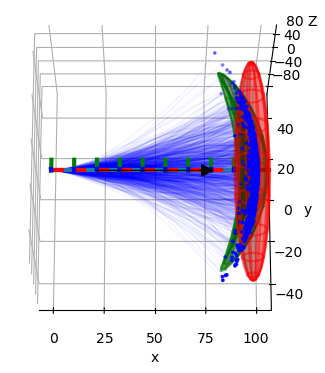
\includegraphics[width=0.4\textwidth]{images/state_estimation}\end{center}
\vskip -0.4cm
The \textbf{banana distribution} is Gaussian in exponential coordinates:
\[
\boldsymbol{T} = Exp(\mathcal{S}\theta) \overline{\boldsymbol{T}},\quad \textrm{with} \quad \mathcal{S}\theta \sim \mathcal{N}\left(\boldsymbol{0}, \boldsymbol{\Sigma}_{6 \times 6}\right)
\]
\parencite{Long2012,Barfoot2014}
\end{frame}

\begin{frame}[fragile]{Concatenation of Uncertain Transforms}
\begin{lstlisting}[language=Python]
import pytransform3d.uncertainty as pu
# estimated mean pose (transformation matrix)
T_est = ...
# covariance in exponential coordinates
cov_est = ...
# mean offset (transformation matrix)
T_vel = ...
# covariance in exponential coordinates
cov_vel = ...

T_est, cov_est = pu.concat_globally_uncertain_transforms(
        T_est, cov_est,
        T_vel, cov_vel)
\end{lstlisting}
\end{frame}

\begin{frame}
\begin{center}
\Large
Application: Transfer of Motions to Robotic Hand
\end{center}
\end{frame}

\begin{frame}[fragile]{Robot Kinematics}
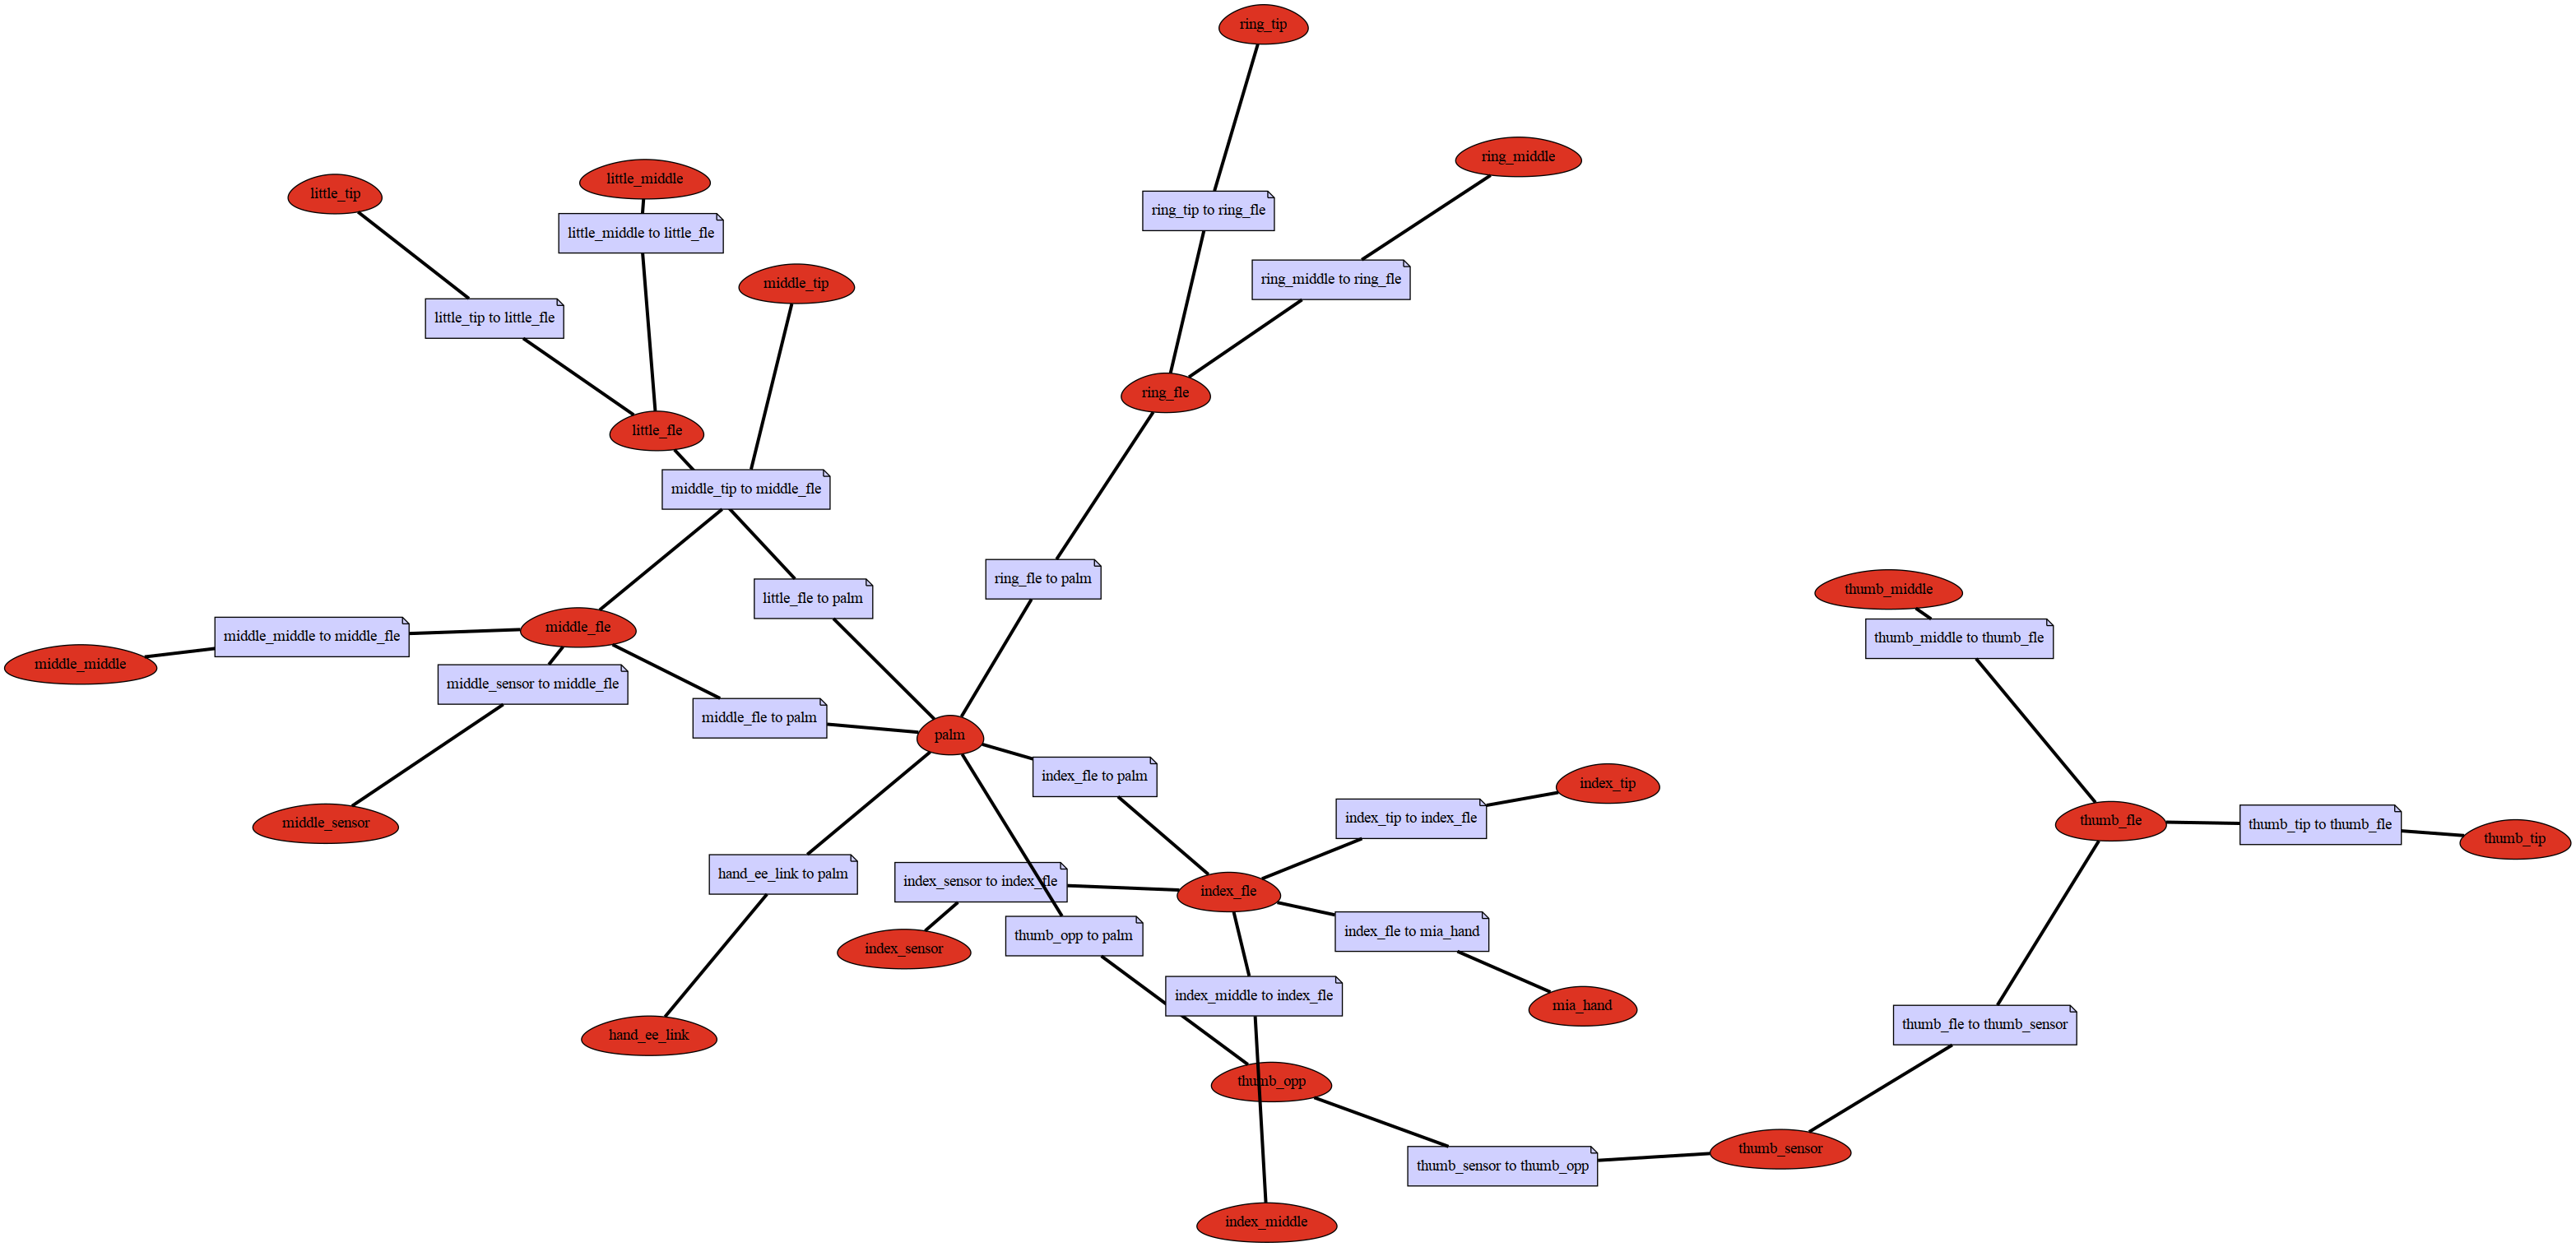
\includegraphics[width=\textwidth]{images/embodiment_graph}
\begin{lstlisting}[language=Python]
from pytransform3d.urdf import UrdfTransformManager
tm = UrdfTransformManager()
with open("robot.urdf", "r") as f:
    robot_urdf = f.read()
tm.load_urdf(robot_urdf)
tm.write_png(graph_filename)
\end{lstlisting}
\end{frame}

\begin{frame}[plain,fragile]{Graphs of Transformations}
Examples: kinematic structures of robots (and other articulated bodies),
estimated states, trajectories

\begin{columns}
\begin{column}{0.4\textwidth}
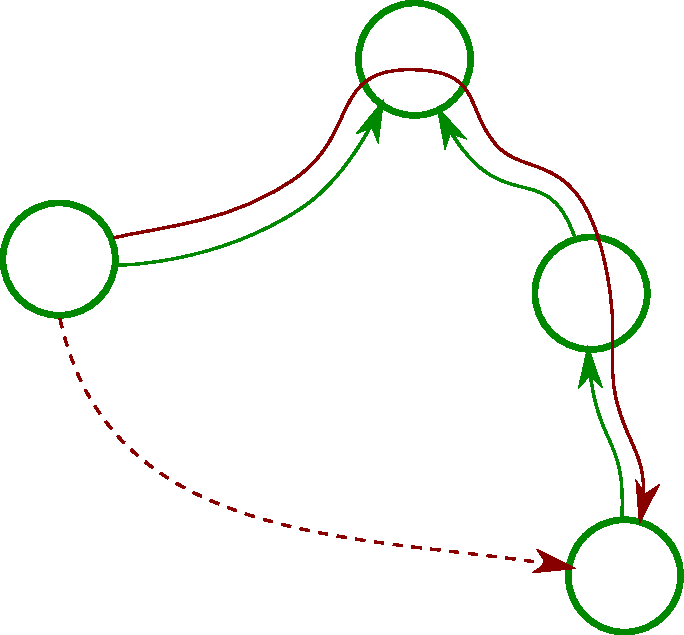
\includegraphics[width=\textwidth]{images/transform_graph}
\end{column}
\begin{column}{0.6\textwidth}
\begin{lstlisting}[language=Python]
from pytransform3d.transform_manager import TransformManager


tm = TransformManager()
tm.add_transform(
    "end-effector", "robot", ee2robot)
tm.add_transform(
    "camera", "robot", cam2robot)
tm.add_transform(
    "object", "camera", object2cam)

ee2object = tm.get_transform(
    "end-effector", "object")
\end{lstlisting}
\end{column}
\end{columns}
\end{frame}

\begin{frame}[fragile]{Transfer of Motions to Robotic Hand}
\begin{columns}
\begin{column}{0.4\textwidth}
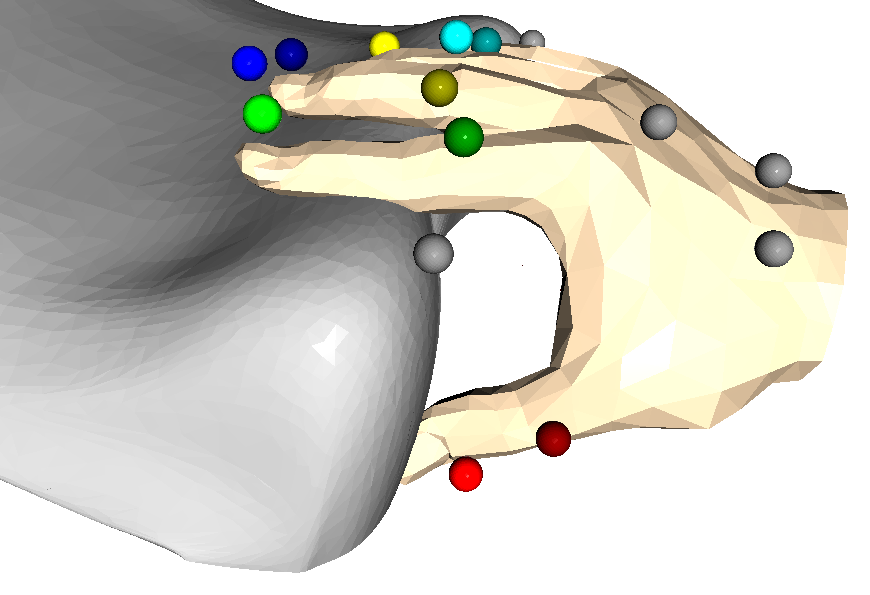
\includegraphics[width=\textwidth]{images/embodiment_record}
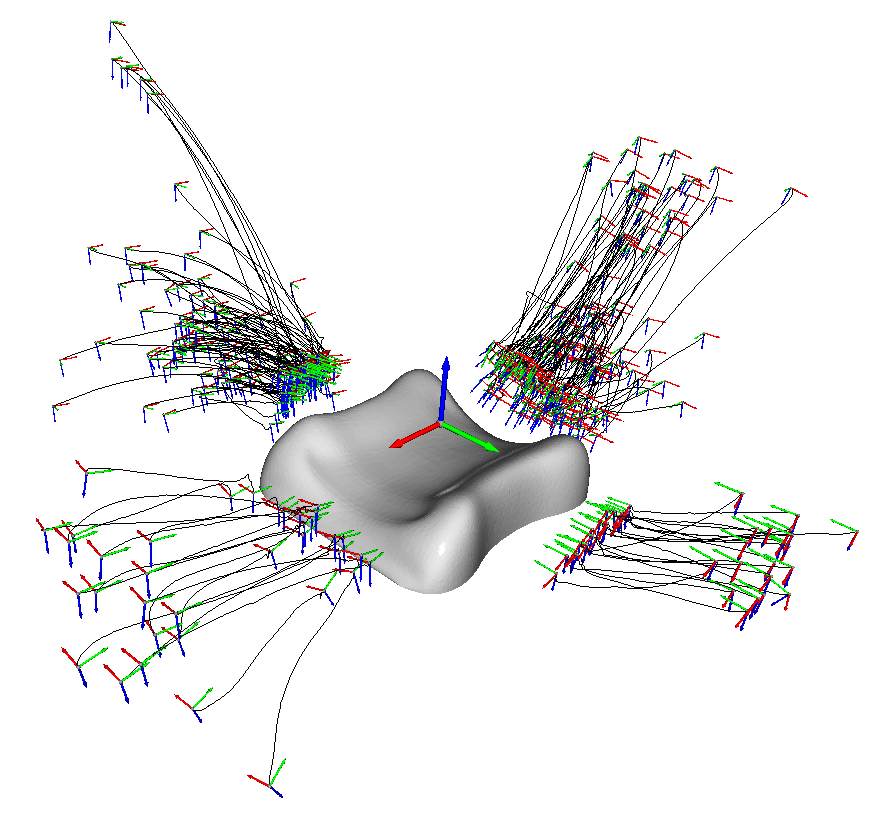
\includegraphics[width=\textwidth]{images/embodiment_dataset}
\end{column}
\begin{column}{0.6\textwidth}
\makebox(165,160){
%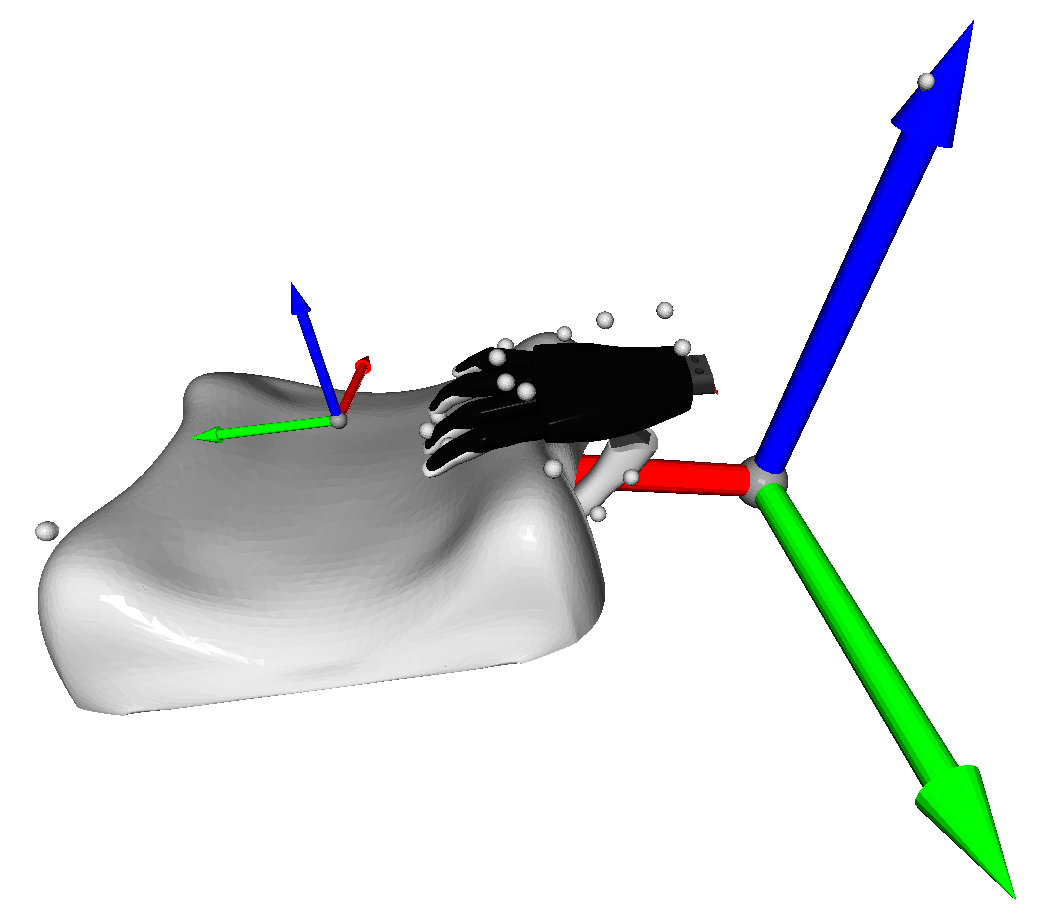
\includegraphics[width=165pt]{images/embodiment_mia}%
\movie[loop,autostart,poster,width=165pt]
{\makebox(165,160){}}
{videos/embodiment.mp4}}%
\end{column}
\end{columns}
{\small \url{https://github.com/dfki-ric/hand_embodiment}, \parencite{Fabisch2022}}
\end{frame}

\begin{frame}
\begin{center}
\Large
Application: Collision Detection
\end{center}
\end{frame}

\begin{frame}{Collision Detection}
\makebox(305,185){
\movie[loop,autostart,poster,width=160pt]
{\makebox(160,185){}}
{videos/collision_detection.mp4}}
\begin{itemize}
\item Broad phase collision detection with AABBs
\item GJK algorithm \parencite{Gilbert1988}
\end{itemize}
\end{frame}

\begin{frame}[fragile]{Collision Detection}
\begin{lstlisting}[language=Python]
from pytransform3d.urdf import UrdfTransformManager
from distance3d import broad_phase


# Load graph of transformations
robot_tree = UrdfTransformManager()
with open(filename, "r") as f:
    robot_urdf = f.read()
robot_tree.load_urdf(robot_urdf)

# Define configuration of robot
for joint_name in ["joint%d" % i for i in range(1, 7)]:
    robot_tree.set_joint(joint_name, 0.7)

# Construct bounding volume hierarchy for broad phase
robot_bvh = broad_phase.BoundingVolumeHierarchy(
    robot_tree, "robot_arm")
robot_bvh.fill_tree_with_colliders(robot_tree)
\end{lstlisting}

\setbeamercolor{boxcolor}{bg=blue!10}
\begin{beamercolorbox}[wd=\textwidth,sep=5pt]{boxcolor}
{\footnotesize Library:
\url{https://github.com/AlexanderFabisch/distance3d}}
\end{beamercolorbox}
\end{frame}

\begin{frame}{Funding}
\begin{center}

\includegraphics[width=0.5\textwidth]{images/logo_april}
\end{center}
This work was supported by the European Commission under the Horizon 2020
framework program for Research and Innovation (project acronym: APRIL, project
number: 870142).
\end{frame}

\begin{frame}{Features of pytransform3d}

\includegraphics[width=\textwidth]{images/logo}

\begin{itemize}
\item \textbf{operations} for most common representations of rotation and translation
\item \textbf{conversions} between representations
\item clear documentation of \textbf{conventions}
\item coupling with \textbf{matplotlib} for quick visualization
\item the TransformManager organizes complex \textbf{graphs of transformations}
\item a matplotlib-like interface to Open3D’s \textbf{visualizer}
\end{itemize}
\end{frame}

\begin{frame}
\begin{center}
\Large
Backup
\end{center}
\end{frame}

\begin{frame}[plain,fragile]{Modeling Transformations}
\textbf{Mathematical notation:}
$\boldsymbol{T}_{BA}$ for transformation \textit{from frame} \texttt{A} \textit{to frame}
\texttt{B}. In concatenation, read from right to left:

\[
\boldsymbol{T}_{CB} \boldsymbol{T}_{BA} = \boldsymbol{T}_{C\cancel{B}} \boldsymbol{T}_{\cancel{B}A} = \boldsymbol{T}_{CA}.
\]

\vfill

\textbf{In code} we should prefer the notation \texttt{A2B}
for a transformation \textit{from frame} \texttt{A} \textit{to frame} \texttt{B}:

\begin{lstlisting}[language=Python]
from pytransform3d.transformations import concat
A2B = ...  # transformation from frame A to frame B
B2C = ...  # transformation from frame B to frame C
A2C = concat(A2B, B2C)
\end{lstlisting}
\end{frame}

\begin{frame}[fragile]{Imitation Learning}
\makebox(300,200){
\movie[loop,autostart,poster,width=150pt]
{\makebox(200,200){}}
{videos/dual_arm.mp4}}
\end{frame}

\begin{frame}[t,allowframebreaks]{Literature}
\printbibliography[heading=none]
\end{frame}

\end{document}
